\documentclass[10pt]{article}
\usepackage[letterpaper,margin=0.55in,top=0.42in,bottom=0.38in]{geometry}
\usepackage{fontspec}
\setmainfont{TeX Gyre Termes}
\setmonofont{TeX Gyre Cursor}[Scale=0.95]
\usepackage{amsmath,booktabs,graphicx,microtype}
\usepackage[font=small,labelfont=bf,skip=3pt]{caption}
\usepackage{titlesec}
\titleformat{\section}{\normalsize\bfseries}{\thesection\quad}{0pt}{}
\titlespacing*{\section}{0pt}{4pt}{0pt}
\usepackage{enumitem}
\setlist{nosep,leftmargin=1.4em,topsep=1pt}
\usepackage[hidelinks,pdftitle={Does event-JEPA pretraining beat its own random initialisation?},pdfauthor={Siddhant Shankar}]{hyperref}
\setlength{\parindent}{0pt}
\setlength{\parskip}{3pt}
\pagestyle{empty}
\newcommand{\code}[1]{\texttt{#1}}

\begin{document}

{\Large\bfseries Does event-JEPA pretraining beat its own random initialisation?}\\[3pt]
{\normalsize A one-page proposal on scaling HEPA/KITE}\\[1pt]
{\small Siddhant Shankar \;·\; University of Illinois Urbana-Champaign \;·\; \href{mailto:ss284@illinois.edu}{ss284@illinois.edu} \;·\; November 2026}

\vspace{-2pt}
\section{Motivation}
HEPA [1] pretrains a causal Transformer with a horizon-conditioned JEPA objective, freezes it, and finetunes the predictor into a monotone survival CDF. KITE [2] keeps that backbone and makes the encoder channel-agnostic. Growing either into a foundation model assumes the frozen pretrained encoder knows something the same architecture does not know at initialisation; in time-series classification, ROCKET [4] showed random features with a linear head are hard to beat. I tested it on the public code first.

\section{Pilot: pretrained vs.\ never-trained encoder}
I ran the repository's \code{scripts/train.py} at its PROTOCOL defaults ($d{=}256$, 2.16M parameters, 50/30 epochs) with \code{--pre-epochs 50} and \code{--pre-epochs 0}; the latter leaves the encoder at initialisation (checked by hash) and runs the same finetuning code. Pretrained FD001 reaches 0.901, against the $\sim$0.902 the repository's \code{REPRODUCIBILITY.md} says to expect.

\begin{center}
\small
\captionof{table}{Mean per-horizon AUROC (the repository's \code{h\_auroc}), mean $\pm$ sd over 3 seeds; $\Delta$ is paired.}
\vspace{-2pt}
\begin{tabular}{lccccc}
\toprule
 & FD001 & FD003 & MBA & PSM & ETTm1 \\
\midrule
Random encoder, never trained & $.924 \pm .002$ & $.957 \pm .002$ & $.799 \pm .051$ & $.631 \pm .008$ & $.812 \pm .010$ \\
Pretrained encoder (published recipe) & $.901 \pm .007$ & $.941 \pm .003$ & $.820 \pm .010$ & $.629 \pm .022$ & $.809 \pm .011$ \\
$\Delta$ (pretrained $-$ random) & $-.0225 \pm .0063$ & $-.0155 \pm .0056$ & $+.0210 \pm .0430$ & $-.0022 \pm .0139$ & $-.0029 \pm .0172$ \\
Seeds where pretrained is ahead & 0/3 & 0/3 & 2/3 & 1/3 & 1/3 \\
\bottomrule
\end{tabular}
\end{center}
\vspace{-4pt}

On both C-MAPSS subsets the never-trained encoder is better in every seed; on MBA, PSM and ETTm1 the two are within seed noise. Figure~1a locates the deficit: re-initialising the predictor on top of the pretrained encoder leaves it in place, while putting the pretrained predictor on a random encoder removes it, so it lives in the encoder. Over pretraining, the centred effective rank of the target embeddings falls from about 13 to 1.3 (mean pairwise cosine $0.65 \to 0.999$). A variance--covariance penalty on the targets raises their rank to 40--54 and closes most of the gap, but does not put pretraining ahead of random. Widening the model does not close it either (Fig.~1b): pretraining trails random in 17 of 18 C-MAPSS seed $\times$ width runs. Earlier, at a reduced budget, sharing one encoder across all five datasets cost 0.017 mean pooled AUROC (0.823 vs.\ 0.840) and the same target penalty recovered it (0.839, two seeds).

\vspace{-2pt}
\begin{center}
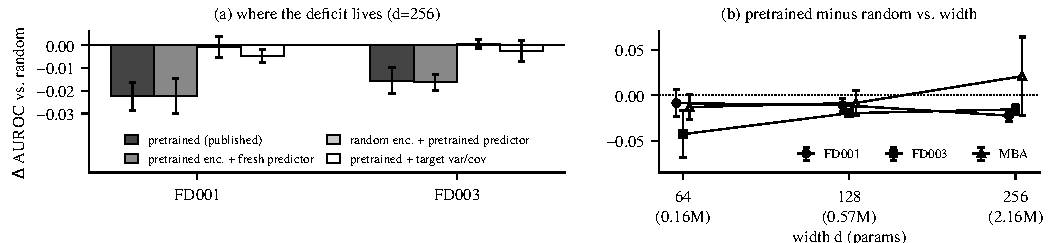
\includegraphics[width=0.78\linewidth]{fig_mechanism.pdf}
\captionof{figure}{Per-horizon AUROC minus the never-trained encoder's (paired, mean $\pm$ sd, 3 seeds). (a) Encoder/predictor swap and target penalty. (b) Width sweep.}
\end{center}
\vspace{-8pt}

\section{Hypothesis}
\textit{Event-JEPA pretraining adds value over the untrained architecture only when the target is kept from collapsing and the corpus spans many domains. At per-dataset scale the pretrained encoder is no better than its own initialisation; as data and model grow together, the pretrained-minus-random gap turns positive only with a target-side regulariser.}
Refuted if (a) under the configuration behind the paper's table (detached target, SIGReg, 100/50 epochs) pretraining beats random by more than one seed-sd on most of the 14 benchmarks; (b) at 10--40M parameters on FactoryNet [3] plus the 14 benchmarks the gap stays $\le 0$ even with SIGReg on the targets; or (c) it turns positive with no target-side regulariser.

\section{Plan}
(1) \textit{CPU, $\sim$6--8 core-hours:} The detached-target configuration, a pretraining-length sweep (0/5/15/50 epochs), and FD002/FD004. (2) \textit{One GPU, est.\ 20--60 A10G-hours:} All 14 benchmarks $\times$ 5 seeds $\times$ \{published objective, random encoder, target var/cov, SIGReg, frozen target\}, plus $d{=}512$ and 1024. Outcome (a) ends the project here. (3) \textit{Forgis compute, est.\ 190--750 GPU-hours:} FactoryNet plus the 14 benchmarks with KITE variate tokens; three objectives $\times$ three seeds $\times$ \{2M, 10M, 40M\}. The random control needs only finetunes. (GPU-hours extrapolated from measured CPU cost, 472 core-s/run; least certain input: KITE's mean variate count.) For the 2027 papers the by-product is an evaluation row, ``same architecture, never trained'', which costs one finetune and turns ``the pretrained model beats baselines'' into ``pretraining added this much''. Where that gap turns positive is a result either way.

\textbf{Limitations.} 2-core CPU; five of fourteen benchmarks; three seeds on a fixed split. The public code is not the paper's run (VICReg-style regulariser, joint target, 50/30 epochs), so none of this speaks to the published numbers. Both clear losses are on C-MAPSS (global z-scoring, no RevIN), which may favour random projections; MBA, PSM and ETTm1 get at most 50 pretraining steps.

{\small Code and per-run results: \href{https://github.com/Siddhant-Shankar/Siddhant_Shankar_HEPA_KITE_Proposal}{github.com/Siddhant-Shankar/Siddhant\_Shankar\_HEPA\_KITE\_Proposal}. \ [1] HEPA, arXiv:2605.11130; [2] KITE, arXiv:2610.12738; [3] FactoryNet, arXiv:2605.09081; [4] Dempster et al., ROCKET, DMKD 2020.}

\end{document}
